\documentclass[tikz,border=8pt]{standalone}

\usepackage{xcolor}
\usepackage{tikz}

% -----------------------
% Color definitions
% -----------------------
\definecolor{varred}{RGB}{200,0,0}
\definecolor{lightbluebg}{RGB}{240,245,255} % faint bluish

\begin{document}

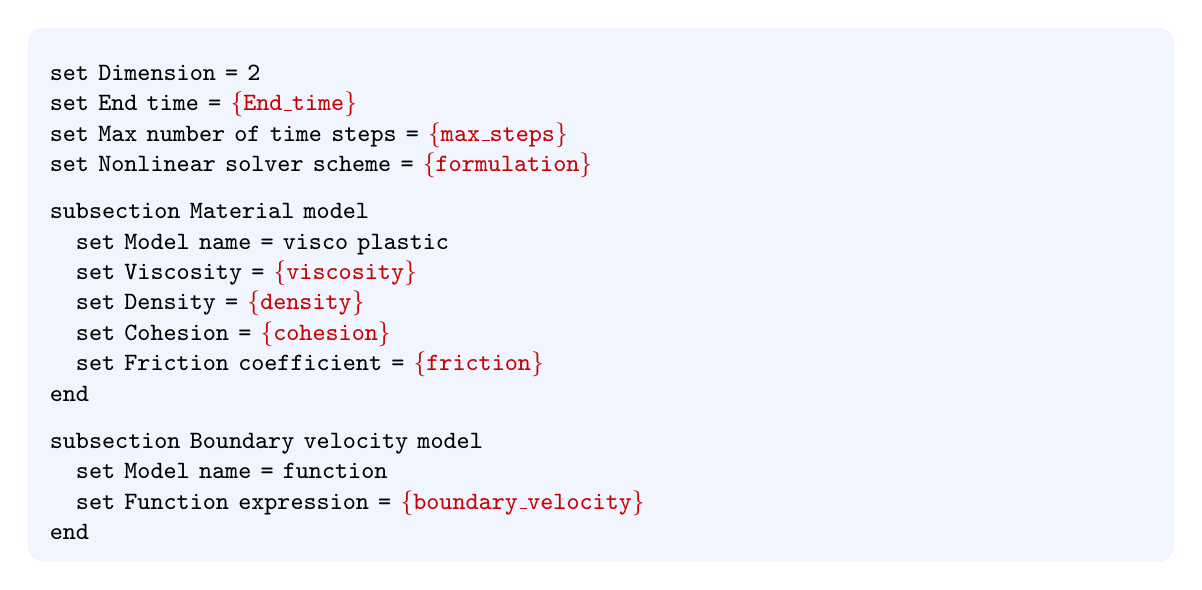
\begin{tikzpicture}

\node[
    fill=lightbluebg,
    rounded corners=6pt,
    inner sep=8pt,
    text width=14cm
] (box)
{
\ttfamily\small

set Dimension = 2 \\
set End time = \textcolor{varred}{\{End\_time\}} \\
set Max number of time steps = \textcolor{varred}{\{max\_steps\}} \\
set Nonlinear solver scheme = \textcolor{varred}{\{formulation\}} \\[6pt]

subsection Material model \\
\quad set Model name = visco plastic \\
\quad set Viscosity = \textcolor{varred}{\{viscosity\}} \\
\quad set Density = \textcolor{varred}{\{density\}} \\
\quad set Cohesion = \textcolor{varred}{\{cohesion\}} \\
\quad set Friction coefficient = \textcolor{varred}{\{friction\}} \\
end \\[6pt]

subsection Boundary velocity model \\
\quad set Model name = function \\
\quad set Function expression = \textcolor{varred}{\{boundary\_velocity\}} \\
end

};

\end{tikzpicture}

\end{document}